% NOTE: paired with figures/03_dgm_archive.tex — see the note there and
% paper/supplementary/source-attribution.md.
\begin{figure}[ht]
\centering
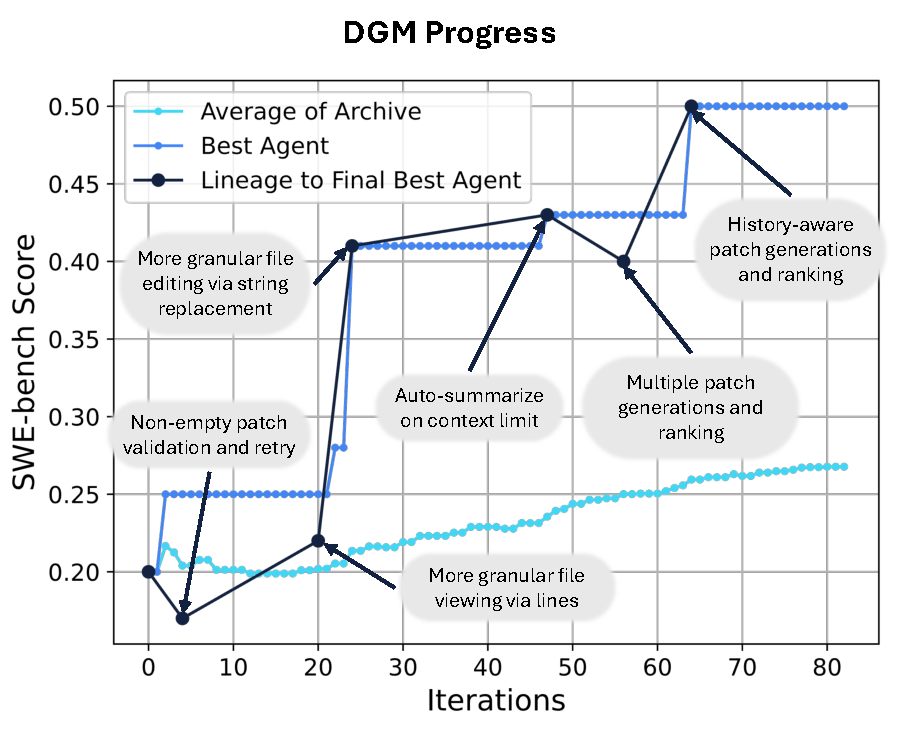
\includegraphics[width=0.9\textwidth]{figures/srcs/04_dgm_progress.pdf}
\caption{\textbf{The DGM automatically self-improves to become a better coding agent.} (Left) Archive of coding agents generated during the DGM run on SWE-bench, see \Cref{fig:dgm-archive}. (Right) Progress plot of the DGM on SWE-bench. The light blue line shows the average score of all agents possessing basic codebase-editing functionality. The blue line tracks the best score achieved by any agent in the archive at each iteration. The dark line shows the lineage of the final best-discovered agent and its precursor nodes, which includes two performance dips. This illustrates the benefits of open-ended search, which explores a diverse set of interesting stepping stones instead of focusing only on branching off the best solution found so far.}
\label{fig:dgm-progress}
\end{figure}
